
In this Chapter we implement a finite element method (FEM) for an unstructured triangular mesh on a general polygonal domain.  Our code solves certain linear and nonlinear Poisson equation problems with reasonably-general boundary conditions.  The approach is to
\begin{center}
\emph{first do element-wise assembly of the residual equations,}
\end{center}
and thereby get a functioning \pSNES-based code.  We will not even think about matrices in writing the initial code.  Only after making sure it works do we
\begin{center}
\emph{write additional code to assemble an approximate Jacobian matrix.}
\end{center}

We do the following new tasks in this Chapter:
\begin{itemize}
\item read a triangular mesh from a file into \PETSc \pVecs and \pISs,
\item index that mesh unstructured way,
\item pre-allocate a \PETSc \pMat, and
\item implement Neumann boundary conditions.
\end{itemize}

Similarly to the example in the last Chapter, the residual equations $\bF(\bu)=0$, which is to say the nonlinear system seen by the \pSNES solver, is the discretized weak form of the PDE.  Our direct construction of these equations roughly follows the residual implementations of Chapters \ref{chap:nl}--\ref{chap:of}.

The FEM ``stiffness'' matrix $A$, a major piece in typical FEM introductions \citep{Braess2007,Elmanetal2005}, arises here as the Jacobian when solving $\bF(\bu)=0$.  In our first runs, done before writing any matrix-assembly code, the \pSNES solver approximates this linear system through finite-differencing evaluations of $\bF$.  Eventually we do assemble a Jacobian, but one that is only correct for the linear case.  For the smooth nonlinear case tested here, however, this inaccurate linearization suffices.

The example here contrasts with the rectangular-element ($Q^1$) FEM of the last Chapter by not using a \pDMDA and a structured grid.  Instead we implement a minimal, though naive, mesh-topology infrastructure.  (Doing so substantially increases our workload!)  The relatively-simple \Triangle program generates ASCII files describing the mesh.  An ``index set'' \pIS  type holds the global indices of nodes and triangles (elements).  \pVec and \pMat objects, used for the solution and Jacobian respectively, are indexed through the \pIS values.

In contrast with both earlier and later Chapters, we generate a code that only works on one MPI process (i.e.~a serial code).  However, at the end of the Chapter we briefly consider, though we do not implement, the additional constructs needed to distribute a mesh across many processes.  These considerations motivate the \pDMPlex example in Chapter \ref{chap:dp}.  In fact, the benefits of \PETSc's mesh-topology \pDM tools, including \pDMDA in previous Chapters and \pDMPlex in Chapter \ref{chap:dp}, become clearer by forgoing them here.


\section{A 2D nonlinear Poisson problem}

\begin{marginfigure}
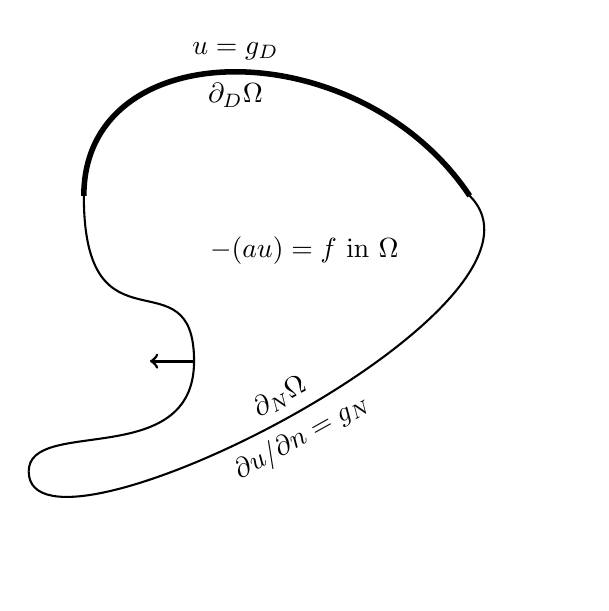
\begin{tikzpicture}[scale=0.7]
%\draw[gray,very thin] (-2,-6) grid (8,3);
\draw[line width=2pt] (0,0) .. controls (0,3) and (5,3) .. node[sloped,above] {$u=g_D$} node[sloped,below] {$\partial_D\Omega$} (7,0);
\draw[line width=0.75pt] (7,0) .. controls (9,-2) and (-1,-7) .. node[sloped,above] {$\partial_N\Omega$} node[sloped,below] {$\partial u/\partial n = g_N$} (-1,-5);
\draw[line width=0.75pt] (-1,-5) .. controls (-1,-4) and (2,-5) .. (2,-3);
\draw[line width=0.75pt] (2,-3) .. controls (2,-1) and (0,-3) .. (0,0);
\draw[->,line width=1.0pt] (2,-3) -- (1.2,-3) node[below] {$\bn$}; % normal vector
\draw (4,-1) node {$- \Div (a \grad u) = f$ in $\Omega$};
\end{tikzpicture}


\caption{Problem \eqref{eq:un:poissonstrong} on a domain.}
\label{fig:un:generalpoissondomain}
\end{marginfigure}

Let $\Omega \subset \RR^2$ be a bounded (open) region as in Figure \ref{fig:un:generalpoissondomain}.  We suppose its boundary $\partial\Omega$ is well-behaved, for example polygonal or Lipschitz-continuous \citep[section 1.2]{Ciarlet2002}.  Also we decompose the boundary into (measurable) disjoint subsets $\partial_D \Omega$ and $\partial_N \Omega$.

Chapter \ref{chap:st} solves the Poisson equation $- \grad^2 u = f$.  Here we allow a more general nonlinear form.  Let $a(u,x,y)$ and $f(u,x,y)$ be continuous functions, and assume there is $\eps$ so that
\begin{equation}
a(u,x,y) \ge \eps > 0, \label{eq:un:uniformelliptic}
\end{equation}
that is, \emph{uniform ellipticity} \citep{Evans2010}.  Boundary conditions are also needed, and here we consider nonhomogeneous Dirichlet and Neumann type.  Thus the  nonlinear Poisson \emph{strong form} we solve is to find $u(x,y)$ so that
\begin{align}
- \Div \left(a(u,x,y) \grad u\right) &= f(u,x,y) \quad \text{ on } \Omega, \label{eq:un:poissonstrong} \\
u &= g_D \quad \text{ on } \partial_D \Omega, \notag \\
\frac{\partial u}{\partial n} &= g_N \quad \text{ on } \partial_N \Omega. \notag
\end{align}
By definition, $\partial u/\partial n = \bn \cdot \grad u$ where $\bn$ is the outward unit normal on $\partial \Omega$ (Figure \ref{fig:un:generalpoissondomain}).

The data of problem \eqref{eq:un:poissonstrong}, besides the region $\Omega$ and its boundary, includes a \emph{diffusion coefficient} $a$, a \emph{source term} $f$, \emph{Dirichlet data} $g_D$, and \emph{Neumann data} $g_N$.  For the purpose of numerical solutions we will assume these data are continuous.  Poisson problem \eqref{poissonsquare} in Chapter \ref{chap:st} is the homogeneous Dirichlet case where $\Omega$ is a square, $a\equiv 1$, $f=f(x,y)$, $\partial_D \Omega = \partial \Omega$, $\partial_N \Omega = \emptyset$, and $g_D=0$.

One could allow more general boundary conditions in \eqref{eq:un:poissonstrong}, in particular \emph{Robin} conditions $\alpha u + \beta \frac{\partial u}{\partial n} = \gamma$ where $\alpha,\beta,\gamma$ could vary along the boundary \citep{Elmanetal2005}; see Exercise \ref{chap:un}.\ref{exer:un:robin}.  One could also allow $a$ and/or $f$ to depend on the gradient of $u$; recall $a=|\grad u|^{p-2}$ in the $p$-Laplacian equation of Chapter \ref{chap:of}, for example.

As \eqref{eq:un:poissonstrong} is stated there may be no solution where ``$\Div(a\grad u)$'' makes sense as a continuous function, even for polygonal regions and continuous data.  That is, there may be no $u\in C^2(\Omega) \cap C(\overline \Omega)$ so that \eqref{eq:un:poissonstrong} applies at all points.  In the linear case, at least, a solution exists if we convert \eqref{eq:un:poissonstrong} to a \emph{weak form}.  Such a weak formulation already arose in Chapter \ref{chap:of} as the gradient of an objective function, but the weak form here generally does not have a minimization origin; see Exercise \ref{chap:un}.\ref{exer:un:notminimization}.  In this Chapter we will derive the weak form from the strong form in the traditional way, by multiplying by a test function and integrating.


\section{Weak form with general boundary values}

Recall $L^2(\Omega)$ is the space of square-integrable real functions on $\Omega$.  Define the following Hilbert space:
    $$H^1(\Omega) = \left\{u \,:\, u \in L^2(\Omega) \,\&\, \grad u \in L^2(\Omega)\right\}.$$
Definition \eqref{eq:of:sobolevdefn} of Sobolev spaces $W^{1,p}(\Omega)$ includes this space: $H^1(\Omega) = W^{1,2}(\Omega)$.

We use two subsets of $H^1(\Omega)$: \emph{trial functions} come from $H_{g}^1(\Omega)$, the functions with value $g_D$ along $\partial_D \Omega$, and \emph{test functions} come from $H_{0}^1(\Omega)$, with value $0$ along $\partial_D \Omega$.  Note that $H_{0}^1(\Omega)$ is a linear subspace of $H^1(\Omega)$ while generally $H_{g}^1(\Omega)$ is not.

Now choose any $v\in H_{0}^1(\Omega)$, multiply the first equation in \eqref{eq:un:poissonstrong} by $v$, and integrate by parts:
\begin{equation*}
\int_\Omega a(u) \grad u \cdot \grad v - \int_{\partial\Omega} \frac{\partial u}{\partial n} v = \int_\Omega f(u) v.
\end{equation*}
In writing such integrals we will generally show dependence on the solution $u$ but suppress it for $x,y$ so that $a(u,x,y)=a(u)$, and similarly for $f$.

Next we use the boundary information, that $v=0$ on $\partial_D\Omega$ and $\partial u/\partial n=g_N$ on $\partial_N\Omega$:
\begin{equation}
\int_\Omega a(u) \grad u \cdot \grad v = \int_\Omega f(u) v + \int_{\partial_N\Omega} g_N v\quad \text{ for any } v\in H_{0}^1(\Omega). \label{eq:un:poissonweak}
\end{equation}
Equation \eqref{eq:un:poissonweak} is the \emph{weak formulation} of \eqref{eq:un:poissonstrong}.  Any $u \in H_{g}^1(\Omega)$ satisfying \eqref{eq:un:poissonweak} is a \emph{weak solution}.  Observe that the Dirichlet boundary conditions $g_D$ are incorporated into defining $H_{g}^1(\Omega)$ while the Neumann boundary data $g_N$ appears in the weak form \eqref{eq:un:poissonweak}.

Here are the ``rules'' for passing between the strong \eqref{eq:un:poissonstrong} and weak \eqref{eq:un:poissonweak} formulations:\begin{itemize}
\item A well-behaved function $u \in C^2(\Omega) \cap C(\overline \Omega)$ which satisfies \eqref{eq:un:poissonstrong} also solves \eqref{eq:un:poissonweak}.  The derivation above shows this.
\item If $u \in H_{g}^1(\Omega)$ solves \eqref{eq:un:poissonweak} then we accept it, by definition, as a solution.   If it is also well-behaved, $u \in C^2(\Omega) \cap C(\overline \Omega)$, then we may reverse the derivation to show it solves \eqref{eq:un:poissonstrong}.
\end{itemize}

For the linear case, where functions $a$ and $f$ are independent of $u$, the theory is relatively complete.  If $\partial_D \Omega$ has positive measure then it is a theorem that a solution to \eqref{eq:un:poissonweak} exists and is unique (\emph{well-posedness}; \citep{Ciarlet2002,Evans2010}).  Furthermore there exist conditions on the domain (e.g.~it is a convex polygon) and the boundary data, from which one can show that $u$ solving \eqref{eq:un:poissonweak} is in $C^2(\Omega) \cap C(\overline \Omega)$ (\emph{regularity}; \citep{Evans2010}).  Such theoretical matters are, however, beyond our scope.

In nonlinear cases each particular problem must be analyzed for well-posedness.  In terms of practical computation, however, some nonlinear cases are covered by our method and are solvable using our code.  These include the 2D versions of
\begin{itemize}
\item the \emph{Bratu} equation wherein $a\equiv 1$ and $f=\lambda e^u$, and
\item ``uniformized'' \emph{porous medium} equations \citep{Ockendonetal2003}, in which, for example, $a=u^{m-1}+\eps$ for some $m\ge 1$ and $\eps>0$.
\end{itemize}
For the former see Exercise \ref{chap:un}.\ref{exer:un:bratu}.\sidenote{Exercise \ref{chap:nl}.\ref{exer:nl:bratu} solves the 1D version.}  We will test our code on an easy case of the latter, namely with $a(u)=1+u^2$; see the exact solution \eqref{eq:un:exactsolution} in ``case 1,'' later in this Chapter.


\section{A $P^1$ finite element method}

Our FEM for the Poisson problem requires weak formulation \eqref{eq:un:poissonweak} to be true for $u$ from a finite-dimensional subspace of $H_{g}^1(\Omega)$, and for all test functions $v$ in a finite-dimensional subspace of $H_{0}^1(\Omega)$.  In the \emph{Galerkin} method here, these subspaces, both built from a triangulation of $\Omega$, are nearly the same.

We require $\Omega$ to be polygonal, so that $\partial\Omega$ is a closed polygon (Figure \ref{fig:un:polygon}), and we require that the segments forming $\partial\Omega$ are either entirely in $\partial_D\Omega$ or entirely in $\partial_N\Omega$.  Furthermore we assume $\partial_D\Omega$ is closed and contains at least one segment of positive length, leading to well-posedness of the continuum problem, at least in the linear case.

\begin{marginfigure}
\input{tmp/blob.tikz}
\caption{A polygonal domain $\Omega$.  The Dirichlet portion of the boundary $\partial_D\Omega$ is shown in bold.}
\label{fig:un:polygon}
\end{marginfigure}

By definition, a \emph{triangulation} is a finite set of non-overlapping, non-empty open triangles $\triangle_k$ which tile $\Omega$:
\begin{equation}
\Th = \left\{\triangle_k \,\Big|\, \cup_k \overline{\triangle}_k = \overline{\Omega} \, \text{ and} \,\, \triangle_k \cap \triangle_l = \emptyset \, \text{ if } k\ne l\right\}. \label{eq:un:triangulation}
\end{equation}
Let $K$ be the number of triangles, which are indexed $k=0,\dots,K-1$.  The $N$ nodes are located at $\bx_i=(x_i,y_i)$ for $i=0,\dots,N-1$.  (In contrast to many references, such as \citet{Elmanetal2005} which we follow in many ways, numbering here is zero-based, suitable for a C implementation.)  An example triangulation $\Th$ is shown in Figure \ref{fig:un:number-mesh}.  The subscript ``$h$'' in ``$\Th$'' denotes the typical or maximum size $h$ (e.g.~diameter) of the triangles, for now just a reminder of our desired limit $h\to 0$.  

We will use $P^1$ finite elements \citep{Elmanetal2005}, and thus the functions in use are continuous on the whole of $\overline\Omega$ while being linear on each triangle $\triangle_k$.  Such functions have three degrees of freedom on each $\triangle_k$, which one may think of as the coefficients in the linear formula $a + b x + c y$.  In fact there are more convenient local bases than $\{1,x,y\}$, as follows.  For each node $j$ there is a basis (``hat'') function  $\psi_j(x,y)$ which is linear on each triangle, continuous on all of $\overline{\Omega}$, and equal to one at only one node $j$,
\begin{equation*}
\psi_j(\bx_i) = \delta_{ij}.
\end{equation*}
See Figure \ref{fig:un:hatfunction} and compare Figure \ref{fig:of:q1hat}.  Functions $\psi_j$ are in $H^1(\Omega)$ \citep{Braess2007}, with piecewise-constant partial derivatives $\partial\psi_j/\partial x$ and $\partial\psi_j/\partial y$.  The set $\{\psi_j\}_{j=0,\dots,N-1}$ is linearly-independent.

\begin{marginfigure}
\input{tmp/blob.1.elenum.tikz}

\medskip

\input{tmp/blob.1.nodenum.tikz}
\caption{A triangulation of the polygon in Figure \ref{fig:un:polygon}, with element (top) and node (bottom) numbering.  There are $K=15$ elements, $N=13$ nodes, and $n_D=4$ nodes in $\partial_D\Omega$.}
\label{fig:un:number-mesh}
\end{marginfigure}

Hat functions allow us to interpolate and extend the Dirichlet data $g_D$ from its nodal values on $\partial_D \Omega$ to the whole of $\overline\Omega$.  We number the $n_D$ nodes which are in the Dirichlet boundary by $\bx_{j_l} \in \partial_D\Omega$ for $l=0,\dots,n_D-1$.  Let $\hat g_D \in C(\overline\Omega)$ be the piecewise-linear interpolant of $g_D$ which has value zero at all the nodes $\bx_j$ which are not in the Dirichlet boundary $\partial_D \Omega$:
\begin{equation}
\hat g_D(x,y) = \sum_{l=0}^{n_D-1} g_D(\bx_{j_l}) \psi_{j_l}(x,y). \label{eq:un:hatgdefine}
\end{equation}

Using \eqref{eq:un:hatgdefine} we can specify the finite-dimensional subspaces used in the method in terms of $\hat g_D$ and the span of certain basis functions $\psi_j$.  First, the \emph{test functions} are zero along $\partial_D \Omega$,
\begin{align*}
S_{0}^h &= \Span\left<\psi_j \,:\, \bx_j \notin \partial_D \Omega\right> = \Span\left<\psi_j \,:\, j \neq j_l\right>.
\end{align*}
Second, the \emph{trial functions} have value $g_D$ along $\partial_D \Omega$,
\begin{equation}
S_{g}^h = \left\{\hat g_D + w \,:\, w \in S_{0}^h\right\}.
\end{equation}
Note that $S_{0}^h$ is a linear subspace of $H_{0}^1(\Omega)$ while $S_{g}^h$ is merely an affine subspace of $H^1(\Omega)$.  Also
\begin{equation}
\dim(S_{0}^h)=\dim(S_{g}^h)=N-n_D.
\end{equation}

\begin{marginfigure}
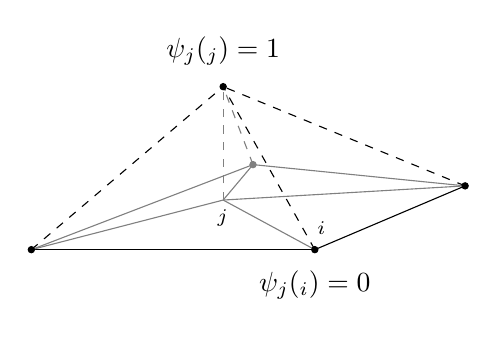
\begin{tikzpicture}[scale=0.9, z={(.707,.3)}]
    % (2,2,1) is top
    \draw[style=dashed] (0,0,0) -- (2,2,1); % to top from left
    \draw[style=dashed] (4,0,0) -- (2,2,1); %   ...  from front
    \draw[style=dashed] (4,0,3) -- (2,2,1); %   ...  from right
    \draw[color=gray, style=dashed] (0.3,0,4) -- (2,2,1); % from back
    \draw[color=gray, style=dashed] (2,0.4,1) -- (2,2,1); % from middle
    % draw base
    \draw (0,0,0) -- (4,0,0);
    \draw (4,0,0) -- (4,0,3);
    \draw[color=gray] (0,0,0) -- (0.3,0,4);
    \draw[color=gray] (0.3,0,4) -- (4,0,3);
    \draw[color=gray] (0,0,0) -- (2,0.4,1);
    \draw[color=gray] (2,0.4,1) -- (4,0,3);
    \draw[color=gray] (4,0,0) -- (2,0.4,1);
    \draw[color=gray] (2,0.4,1) -- (0.3,0,4);
    % draw \psi_j at nodes
    \filldraw (2,2,1) circle (1.25pt);
    \draw (2,2.5,1) node {$\psi_j(\bx_j)=1$};
    \draw (2,0.15,1) node {$\bx_j$};
    \filldraw (0,0,0) circle (1.25pt);
    \filldraw (4,0,0) circle (1.25pt);
    \draw (4,-0.5,0) node {$\psi_j(\bx_i)=0$};
    \draw (4.1,0.3,0) node {$\bx_i$};
    \filldraw (4,0,3) circle (1.25pt);
    \filldraw[color=gray] (0.3,0,4) circle (1.25pt);
\end{tikzpicture}


\caption{Hat functions $\psi_j$.}
\label{fig:un:hatfunction}
\end{marginfigure}

The FEM itself can now be stated.  It requires \eqref{eq:un:poissonweak} to be true for some $u^h\in S_{g}^h$ and for all $v^h\in S_{0}^h$.  By linearity it suffices to consider only a basis of test functions $S_{0}^h$, so we require
\begin{equation}
\int_\Omega a(u^h) \grad u^h \cdot \grad \psi_i = \int_\Omega f(u^h) \psi_i + \int_{\partial_N\Omega} g_N \psi_i \label{eq:un:weakformhat}
\end{equation}
for all $i$ such that $\bx_i \notin \partial_D \Omega$.  On the other hand we may expand $u^h$ using $N-n_D$ unknown coefficients $u_j\in\RR$:
\begin{equation}
u^h(x,y) = \hat g_D(x,y) + \sum_{\bx_j \notin \partial_D \Omega} u_j\, \psi_j(x,y). \label{eq:un:uhexpand}
\end{equation}

The coefficients $u_j$ in \eqref{eq:un:uhexpand} are the unknowns.  Given the triangulation $\mathcal{T}_h$ of $\Omega$ and the data of the problem, namely the functions $a$, $f$, $g_D$, and $g_N$, the complete specification of the FEM solution $u^h$ is given by equations \eqref{eq:un:hatgdefine}, \eqref{eq:un:weakformhat}, and \eqref{eq:un:uhexpand}.

In the linear case it is common to now write system \eqref{eq:un:weakformhat} and \eqref{eq:un:uhexpand} as a linear system $A \bu = \bb$.  The usual next step in an FEM is to assemble the \emph{stiffness matrix} $A$ \citep{Elmanetal2005}.  However, we will not assemble a matrix until we have an initial, and verified, numerical solution.  Following the pattern established since Chapter \ref{chap:nl}, we first implement equation \eqref{eq:un:weakformhat} as a residual-evaluation function $\bF(\bu)$, from the representation of $u^h$ as a vector $\bu$.  In evaluating $\bF$ we use \eqref{eq:un:uhexpand} to get point values of $u^h$ and its gradient $\grad u^h$ on the interior of triangles.  These point values allow quadrature, similar to that in Chapter \ref{chap:of}, to approximate the integrals in \eqref{eq:un:weakformhat}.  Implementing a residual in the linear case is mathematically equivalent to assembling $A$ and $\bb$, but the residual-evaluation code here is simpler because it does not require direct contact with a \PETSc \pMat object at all.

In the next section we describe and the code the element-wise evaluation of the residual function $\bF$ as a \PETSc \pSNES call-back.  However, before the code can be written we need to be more specific about what \eqref{eq:un:weakformhat} says on each element.  Also we will need to read the triangular mesh into \PETSc data structures \pVec and \pIS.  These tools can be tested for correctness with a finite-differenced Jacobian (Chapter \ref{chap:nl}).  Once this is all shown to work correctly, via comparison to an exact solution, then we will consider matrix assembly for the Jacobian.


\section{Assembly of the residual equations}

In expression \eqref{eq:un:uhexpand}, $N-n_D$ values $\{u_j\}$ determine the FEM solution $u^h$.  However, it will be easier to write code if we \emph{increase} the size of the resulting nonlinear system up to dimension $N$ by including the nodal values in the Dirichlet boundary as unknowns:
\begin{equation}
\bu = \{u_j\}_{j=0}^{N-1} \in \RR^N  \label{eq:un:unknowns}
\end{equation}
To enforce the boundary conditions, the components of the residual corresponding to Dirichlet boundary must be zero:
\begin{equation}
F_i(\bu) = u_i - g_D(\bx_i) \qquad \text{ if } \bx_i \in \partial_D\Omega.  \label{eq:un:dirichletresiduals}
\end{equation}

Triangulation $\mathcal{T}_h$ almost\sidenote{The set $\Omega \setminus \cup_k \triangle_k$ has measure zero.} covers $\Omega$ with non-overlapping triangles so we can write the weak form \eqref{eq:un:weakformhat} as a sum over elements.  To be specific, for each $k=0,\dots,K-1$ let
\begin{equation}
F_i^k(\bu) = \int_{\triangle_k} a(u^h) \grad u^h \cdot \grad \psi_i - f(u^h) \psi_i.  \label{eq:un:elementweakform}
\end{equation}
Suppose $n_N$ is the number of segments (edges) which are in the Neumann boundary.  For each segment $s_\nu$, $\nu=0,\dots,n_N-1$, let
\begin{equation}
\varphi_i^\nu = \int_{s_\nu} g_N \psi_i.  \label{eq:un:segmentweakform}
\end{equation}
Note that $\varphi_i^\nu$ does \emph{not} depend on the solution $u^h$.  Then residual equation \eqref{eq:un:weakformhat} is
\begin{equation}
F_i(\bu) = \sum_{k=0}^{K-1} F_i^k(\bu) - \sum_{\nu=0}^{n_N-1} \varphi_i^\nu = 0  \qquad \text{ if } \bx_i \notin \partial_D\Omega. \label{eq:un:elementwisesum}
\end{equation}
Together, equations \eqref{eq:un:dirichletresiduals} and \eqref{eq:un:elementwisesum} form the (generally) nonlinear system, of dimension $N$, which we supply to the \pSNES solver:
\begin{equation}
\bF(\bu)=0. \label{eq:un:fullsystem}
\end{equation}

Observe that $n_D$ is the number of \emph{nodes} in the Dirichlet boundary, whereas $n_N$ is the number of \emph{segments} in the Neumann boundary.  The former are degrees of freedom, while the latter are domains of integration.

Because the support of the hat function $\psi_i$ only overlaps with a few triangles $\triangle_k$, only a few values $F_i^k(\bu)$ and $\varphi_i^\nu$ are nonzero.  Also, only a few nodal values $\bu=\{u_j\}$ enter into $F_i^k(\bu)$, namely those values $u_j$ such that the support of $\psi_j$ overlaps with $\triangle_k$.  These facts make \eqref{eq:un:fullsystem} a sparse nonlinear system.

We will compute the element integrals \eqref{eq:un:elementweakform} by referring $\triangle_k$ to a reference triangle $\triangle_\ast$ with vertices $(0,0),\,(1,0),\,(0,1)$, as shown in Figure \ref{fig:isoparametric}.  (In Chapter \ref{chap:of} we did a similar thing for quadrilaterals.)  If $\triangle_k$ has vertices $(x_0,y_0),\,(x_1,y_1),\,(x_2,y_2)$ then the linear map from $\triangle_\ast$ to $\triangle_k$ is
\begin{align}
x(\xi,\eta) &= x_0 + (x_1-x_0) \xi + (x_2-x_0) \eta, \label{eq:un:trianglemap} \\
y(\xi,\eta) &= y_0 + (y_1-y_0) \xi + (y_2-y_0) \eta. \notag
\end{align}
The Jacobian determinant of this map, which is needed when integrating over the reference element, is constant on each element.  Its magnitude $2|\triangle_k|$ is the ratio of the area $|\triangle_k|$ to the area $|\triangle_\ast|=1/2$.

\begin{marginfigure}
\begin{tikzpicture}[scale=1.1,
    decoration={
      markings,
      mark=at position 1 with {\arrow[scale=1.8,gray]{latex}};
    }]
% left x,y axes
    \draw[->, gray, very thin] (1.5,0) -- (4.0,0);
    \draw[->, gray, very thin] (2,-0.5) -- (2,2.4);
    \draw (4.1,-0.1) node {$x$};
    \draw (1.9,2.4) node {$y$};
    \filldraw (1.7,1) circle (1.25pt);    % (x_0,y_0)
    \filldraw (3.5,-0.3) circle (1.25pt); % (x_1,y_1)
    \filldraw (3.0,2.0) circle (1.25pt);  % (x_2,y_2)
    \draw (1.4,1.3) node {$(x_0,y_0)$};
    \draw (3.5,-0.6) node {$(x_1,y_1)$};
    \draw (3.0,2.3) node {$(x_2,y_2)$};
    \draw[line width=1pt] (1.7,1) -- (3.5,-0.3) -- (3.0,2.0) -- cycle;
    \draw (2.7,1.0) node {$\triangle_k$};
% right xi,eta axes
    \draw[->, gray, very thin] (4.6,0) -- (6.6,0);
    \draw[->, gray, very thin] (5,-0.4) -- (5,2.0);
    \draw (6.7,-0.1) node {$\xi$};
    \draw (4.9,2.05) node {$\eta$};
    \filldraw (5,0) circle (1.25pt);  % (0,0)
    \filldraw (6,0) circle (1.25pt);  % (1,0)
    \filldraw (5,1) circle (1.25pt);  % (0,1)
    \draw (5.2,-0.3) node {$0$};
    \draw (6.2,0.2) node {$1$};
    \draw (5.2,1.1) node {$2$};
    \draw[line width=1pt] (5,0) -- (6,0) -- (5,1) -- cycle;
    \draw (5.3,0.3) node {$\triangle_\ast$};
% arrows connecting nodes
    \draw[gray, postaction={decorate}] (5,0) -- (1.7,1.03);
    \draw[gray, postaction={decorate}] (6,0) -- (3.5,-0.3);
    \draw[gray, postaction={decorate}] (5,1) -- (3.0,2.0);
\end{tikzpicture}


\caption{Mapping of a triangle $\triangle_k$ from the reference triangle $\triangle_\ast$.}
\label{fig:isoparametric}
\end{marginfigure}

On $\triangle_\ast$ any linear function is a linear combination of three local (nodal) basis functions:
\begin{equation}
\chi_0(\xi,\eta) = 1-\xi-\eta, \qquad \chi_1(\xi,\eta) = \xi, \qquad \chi_2(\xi,\eta) = \eta. \label{eq:un:chiformulas}
\end{equation}
If $\bx_i\in\overline{\triangle_k}$ then hat function $\psi_i$ satisfies
\begin{equation}
\psi_i(x(\xi,\eta),y(\xi,\eta)) = \chi_\ell(\xi,\eta) \label{eq:un:psichimap}
\end{equation}
for all $(\xi,\eta)\in\triangle_\ast$, where vertex $\ell \in \{0,1,2\}$ of $\triangle_\ast$ maps to $\bx_i$.

Recalling both the change-of-variables formula for integrals and the chain rule, we can write
\begin{equation}
F_i^k(\bu) = 2 |\triangle_k| \int_{\triangle_\ast} H_\ell^k(\bu,\xi,\eta)\,d\xi\,d\eta \label{eq:un:elementintegralreference}
\end{equation}
where the integrand is
\begin{equation}
H_\ell^k(\bu,\xi,\eta) = \left[a(u^h) \grad u^h \cdot \grad \psi_i - f(u^h) \psi_i\right]_{\triangle_\ast}.  \label{eq:un:elementintegrand}
\end{equation}
Here vertex $\ell$ of $\triangle_\ast$ corresponds to the node $\bx_i$.  Note that ``$\grad$'' in \eqref{eq:un:elementintegrand} refers to derivatives in variables $x,y$.  Exercises \ref{chap:un}.\ref{exer:un:gradientdetails} and \ref{chap:un}.\ref{exer:un:elementintegranddetails} addresses the details implicit in \eqref{eq:un:elementintegralreference} and \eqref{eq:un:elementintegrand}.

As in Chapter \ref{chap:of}, integrals \eqref{eq:un:elementintegralreference} will be approximated using quadrature.  Generally, if there are $Q$ quadrature points $(\xi_q,\eta_q) \in \triangle_\ast$ with weights $w_q$ then
\begin{equation}
F_i^k(\bu) \approx 2 |\triangle_k| \sum_{q=0}^{Q-1} w_q H_\ell^k(\bu,\xi_q,\eta_q). \label{eq:un:elementquadraturereference}
\end{equation}
We use symmetric quadrature rules constructed for the reference triangle $\triangle_\ast$.  (Unsymmetric quadrature rules based on tensor products of one-dimensional integrals \citep{KarniadakisSherwin2013} are an alternative.)  Table \ref{tab:un:quadrature} shows the degree $1,2,3$ Gaussian rules \citep{Dunavant1985} with $Q=1,3,4$ points, respectively (Exercise \ref{chap:un}.\ref{exer:un:checkquadrature}).  Note that the sum of the weights is $1/2$ because $|\triangle_\ast|=1/2$.

\begin{table}[h]
\vspace{0.1in}

\begin{tabular}{lccc}
degree & $Q$ & weights $w_q$ & nodes $(\xi_q,\eta_q)$ \\ \hline
$1$ & $1$ & $1/2$ & $(1/3,1/3)$ \\ \hline
$2$ & $3$ & \begin{tabular}{c}
            $1/6$ \\
            $1/6$ \\
            $1/6$
            \end{tabular} & \begin{tabular}{c}
            $(1/6,1/6)$ \\
            $(2/3,1/6)$ \\
            $(1/6,2/3)$
            \end{tabular} \\ \hline
$3$ & $4$ & \begin{tabular}{c}
            $-27/96$ \\
            $25/96$ \\
            $25/96$ \\
            $25/96$
            \end{tabular} & \begin{tabular}{c}
            $(1/3,1/3)$ \\
            $(1/5,1/5)$ \\
            $(3/5,1/5)$ \\
            $(1/5,3/5)$
            \end{tabular}
\end{tabular}

\vspace{0.1in}
\caption{Symmetric quadrature rules on the reference triangle $\triangle_\ast$.  See \eqref{eq:un:elementquadraturereference}.} \label{tab:un:quadrature}
\end{table}

For the Neumann boundary contributions we use the midpoint rule; compare Exercise \ref{chap:un}.\ref{exer:un:gaussneumann}.  Observe that hat function $\psi_i$ has value $1/2$ at the midpoint of any edge which is incident to $\bx_i$.  If $(x_m,y_m)$ is the midpoint and $|s_\nu|$ is the length of segment $s_\nu$, and if $\bx_i\in \overline{s_\nu}$ then
\begin{equation}
\varphi_i^\nu \approx g_N(x_m,y_m) \psi_i(x_m,y_m) |s_\nu| = \frac{1}{2} |s_\nu|\, g_N(x_m,y_m). \label{eq:un:segmentquadrature}
\end{equation}
Otherwise, if $\bx_i \notin \overline{s_\nu}$, then $\varphi_i^\nu=0$.


\section{Example problems}

Let us set up some simple cases with known exact solutions.  The first two cases both test the implementation of the PDE and of Dirichlet boundary conditions, and homogeneous Neumann boundary conditions, but one problem is linear and the other nonlinear.  An additional case tests the general Neumann boundary condition implementation.  Our goal for these problems is that the measured numerical errors from the FEM will only converge at the theoretical rate $O(h^2)$ if our implementation is correct.

\begin{figure}
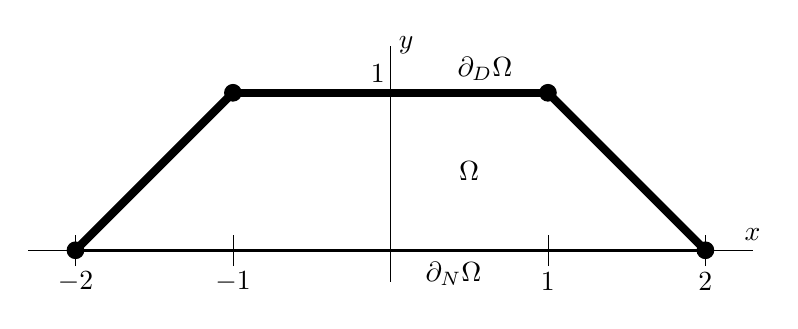
\begin{tikzpicture}[scale=2.000000]
% originally created, in part, by script tri2tikz.py command line:
%   tri2tikz.py --polyonly --nodesize 1.0 --scale 2.0 ../c/ch8/meshes/trap tmp/trap.tikz
% with by-hand edits
  \draw[thin] (0.0,-0.2) -- (0.0,1.3);
  \draw[thin] (-2.3,0.0) -- (2.3,0.0);
  \node at (2.3,0.1) {$x$};
  \node at (0.1,1.3) {$y$};
  \node at (0.5,0.5) {$\Omega$};
  \node at (-0.08,1.12) {$1$};
  \draw[very thin] (-2.0,-0.1) -- (-2.0,0.1);
  \node at (-2.0,-0.2) {$-2$};
  \draw[very thin] (-1.0,-0.1) -- (-1.0,0.1);
  \node at (-1.0,-0.2) {$-1$};
  \draw[very thin] (1.0,-0.1) -- (1.0,0.1);
  \node at (1.0,-0.2) {$1$};
  \draw[very thin] (2.0,-0.1) -- (2.0,0.1);
  \node at (2.0,-0.2) {$2$};
  \node at (0.4,-0.15) {$\partial_N \Omega$};
  \node at (0.6,1.15) {$\partial_D \Omega$};
  \draw[line width=3.0pt] (2.000000,0.000000) -- (1.000000,1.000000);
  \draw[line width=3.0pt] (1.000000,1.000000) -- (-1.000000,1.000000);
  \draw[line width=3.0pt] (-1.000000,1.000000) -- (-2.000000,0.000000);
  \draw[line width=1.25pt] (-2.000000,0.000000) -- (2.000000,0.000000);
  \filldraw (2.0,0.0) circle (1.5pt);
  \filldraw (1.0,1.0) circle (1.5pt);
  \filldraw (-1.0,1.0) circle (1.5pt);
  \filldraw (-2.0,0.0) circle (1.5pt);
\end{tikzpicture}

\caption{Exact solution cases $0$ and $1$ solve Poisson equations on a trapezoidal region $\Omega$.  Boundary subsets $\partial_D\Omega$, $\partial_N \Omega$ are as indicated.  See \texttt{trap.poly} in Code \ref{code:trappoly}.}
\label{fig:un:trap}
\end{figure}

All three cases are based on the same manufactured solution
\begin{equation}
  u_{\text{exact}}(x,y) = 1 - y^2 - \frac{1}{4} y^4. \label{eq:un:exactsolution}
\end{equation}
This formula also computes the Dirichlet boundary values $g_D(x,y)$ in all cases, but other details are case-specific:
\begin{itemize}
\item[case $0$:] \emph{Linear}.  Use Figure \ref{fig:un:trap} boundary conditions.  Noting $\partial u_{\text{exact}}/\partial n = -\partial u_{\text{exact}}/\partial y = 0$ on the Neumann boundary $\partial_N \Omega$, where $y=0$, let $g_N=0$.  Let $a=1$ and determine $f$ by differentiating the exact solution: $f(x,y) = -\grad^2 u_{\text{exact}} = 2 + 3 y^2$.
\item[case $1$:] \emph{Nonlinear}.  Again use Figure \ref{fig:un:trap} boundary conditions and $g_N=0$.  However, let $a(u) = 1+u^2$ and compute the corresponding $f(u)$ by differentiation.
\item[case $2$:] \emph{Non-homogeneous Neumann}.  Use Figure \ref{fig:un:trapneu} boundary conditions.  Let $a$, $f$ be as in case $0$.  Determine the (non-zero) value $g_N$ by differentiating $u_{\text{exact}}$ along the Neumann boundary, a line segment with outward unit normal vector $\bn = \left<1/\sqrt{2},1/\sqrt{2}\right>$.
\end{itemize}
See \texttt{c/\CODELOC cases.h} (not shown) for all remaining details.

\begin{figure}
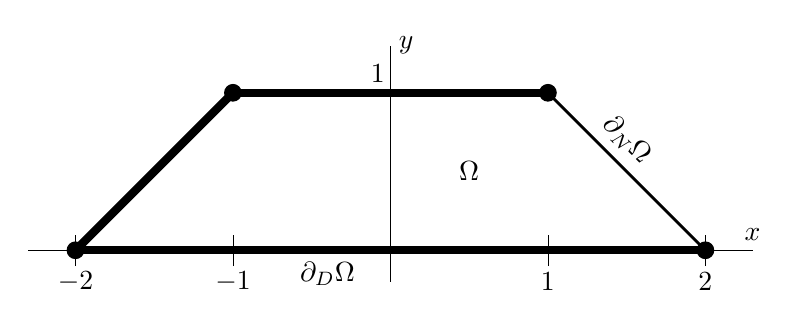
\begin{tikzpicture}[scale=2.000000]
% originally created, in part, by script tri2tikz.py command line:
%   tri2tikz.py --polyonly --nodesize 1.0 --scale 2.0 ../c/ch8/meshes/trap tmp/trap.tikz
% with by-hand edits
  \draw[thin] (0.0,-0.2) -- (0.0,1.3);
  \draw[thin] (-2.3,0.0) -- (2.3,0.0);
  \node at (2.3,0.1) {$x$};
  \node at (0.1,1.3) {$y$};
  \node at (0.5,0.5) {$\Omega$};
  \node at (-0.08,1.12) {$1$};
  \draw[very thin] (-2.0,-0.1) -- (-2.0,0.1);
  \node at (-2.0,-0.2) {$-2$};
  \draw[very thin] (-1.0,-0.1) -- (-1.0,0.1);
  \node at (-1.0,-0.2) {$-1$};
  \draw[very thin] (1.0,-0.1) -- (1.0,0.1);
  \node at (1.0,-0.2) {$1$};
  \draw[very thin] (2.0,-0.1) -- (2.0,0.1);
  \node at (2.0,-0.2) {$2$};
  \node at (-0.4,-0.15) {$\partial_D \Omega$};
  \node[rotate=-45] at (1.5,0.7) {$\partial_N \Omega$};
  \draw[line width=1.0pt] (2.000000,0.000000) -- (1.000000,1.000000);
  \draw[line width=3.0pt] (1.000000,1.000000) -- (-1.000000,1.000000);
  \draw[line width=3.0pt] (-1.000000,1.000000) -- (-2.000000,0.000000);
  \draw[line width=3.0pt] (-2.000000,0.000000) -- (2.000000,0.000000);
  \filldraw (2.0,0.0) circle (1.5pt);
  \filldraw (1.0,1.0) circle (1.5pt);
  \filldraw (-1.0,1.0) circle (1.5pt);
  \filldraw (-2.0,0.0) circle (1.5pt);
\end{tikzpicture}

\caption{Case $2$ uses the same region as in cases $0$ and $1$, but with different boundary conditions.  See \texttt{c/\CODELOC meshes/trapneu.poly} (not shown).}
\label{fig:un:trapneu}
\end{figure}


\section{Triangulations from \Triangle}

\PETSc does not include tools for triangulating regions of the plane, that is, for the initial generation of an unstructured mesh.  We use the widely-available \Triangle\sidenote{See \href{http://www.cs.cmu.edu/~quake/triangle.html}{www.cs.cmu.edu/$\sim$quake/ triangle.html} for documentation.} software \citep{Shewchuk1996} for this task.  \Triangle is limited to 2D, but the ASCII files it generates have straightforward details.

\inputwhole{../c/\CODELOC/meshes/trap.poly}{\CODELOC meshes/trap.poly}{A description of the boundary polygon in Figure \ref{fig:un:trap}, suitable for reading by \Triangle.}{code:trappoly}

\Triangle inputs an ASCII file, with extension \texttt{.poly}, describing a polygonal region $\Omega$ by giving the coordinates of the nodes in $\partial \Omega$.  Integer flags are used indicate special vertices or segments on the boundary.  For example, the input file \texttt{trap.poly} (Code \ref{code:trappoly}) generates the polygon shown in Figure \ref{fig:un:trap}.

The triangulation shown in Figure \ref{fig:un:trapone} came from applying \Triangle to \texttt{trap.poly}, as follows.  We ask for a polygon output file (option \texttt{-p}), relatively-uniform triangles (\texttt{-q} for ``quality-checked,'' with no interior angles less than $20^\circ$ \citep{Shewchuk1996}), and triangles with a maximum area (\texttt{-a}) of $0.5$:
\begin{cline}
$ cd c/ch7/meshes
$ triangle -pqa0.5 trap
\end{cline}
%$
This command generates three ASCII files, \texttt{trap.1.node}, \texttt{trap.1.ele}, and \texttt{trap.1.poly}; see Codes \ref{code:traponenode}--\ref{code:traponepoly}.  They define the new node locations, elements (triples of nodal indices), and segments in the polynomial boundary (pairs of nodal indices), respectively.  This triangulation has $N=8$ nodes, $K=6$ elements, $P=8$ boundary segments, $n_D=5$ Dirichlet nodes, and $n_N=4$ segments in the Neumann boundary.

\begin{figure}
\input{tmp/trap.1.tikz}
\caption{The triangulation described by \texttt{trap.1.\{node,ele,poly\}}.}
\label{fig:un:trapone}
\end{figure}

By giving value ``$2$'' to the Dirichlet nodes in the original \texttt{trap.poly} input, and because \Triangle itself uses ``$0$'' for non-boundary and ``$1$'' for otherwise un-flagged boundary nodes, we have this boundary flag scheme:
\begin{itemize}
\item[0] interior node,
\item[1] Neumann boundary node or segment, and
\item[2] Dirichlet node or segment.
\end{itemize}
Observe that, though \texttt{trap.poly} describes the boundary using only 4 segments, additional boundary nodes and segments have been added in generating the triangulation.

\inputwhole{misc/trap.1.node}{\CODELOC meshes/trap.1.node}{\Triangle-generated ASCII file for node locations and nodal boundary flags.}{code:traponenode}

\inputwhole{misc/trap.1.ele}{\CODELOC meshes/trap.1.ele}{\Triangle-generated ASCII file with element index triples.}{code:traponeele}

\inputwhole{misc/trap.1.poly}{\CODELOC meshes/trap.1.poly}{\Triangle-generated ASCII file for the refined polygon, including segment boundary flags.}{code:traponepoly}

We will test the FEM on a sequence of refined grids generated by \Triangle.  For an example, the command
\begin{cline}
$ triangle -rpqa0.1 trap.1
\end{cline}
%$
generates ASCII files \texttt{trap.2.\{node,ele,poly\}} with $N=33$ nodes, $K=33$ elements, and $P=19$ boundary segments (Figure \ref{fig:un:traptwo}).  Refinement (\texttt{-r}) here means that \emph{nodes} in the \texttt{trap.1} files are retained, but there is no such inclusion relationship for the edges or triangles.  We also see that the symmetry of the \texttt{trap.1} mesh was merely fortuitous.  Symmetries in the input polygon are not preserved by the \Triangle algorithms.

\begin{figure}
\input{tmp/trap.2.tikz}
\caption{A refined triangulation.}
\label{fig:un:traptwo}
\end{figure}

\Triangle includes a minimal visualization tool.  The command
\begin{cline}
$ showme trap
\end{cline}
%$
displays the boundary polygon from \texttt{trap.poly} and all so-far generated levels of the triangulation (\texttt{trap.\{1,2\}.\{node,ele,poly\}}).


\section{Loading the mesh into \PETSc \pVecs and \pISs}

Our plan is to traverse all of the elements $\triangle_k \in \mathcal{T}_h$, and the Neumann boundary segments $s_\nu$, so as to compute the quantities in \eqref{eq:un:elementquadraturereference} and \eqref{eq:un:segmentquadrature}.  The traversal is reasonably fast if the mesh data are stored in \PETSc objects.  We first convert the \Triangle-generated ASCII files into \pVecs and \pISs using a Python script \texttt{tri2petsc.py}.

An abstract description clarifies the way we store the mesh in \PETSc objects.  There are two kinds of ``data'' to describe a mesh, \emph{geometrical} and \emph{topological}.  Here the geometry is simply the nodal locations, pairs of real numbers for each node.  We store these coordinates in a length $2N$ sequential \pVec.  For the topology we have descriptions of which elements (triangles) are incident to which nodes (vertices).  This task only requires integer indices.  The topology of the elements is given by a triple of integers, each node index in the range $0,\dots,N-1$, for each element.  Similarly, a segment of the polygonal boundary is simply a pair of nodal indices identifying the endpoints of segment.

The \PETSc \pIS ``index set'' type is convenient for storing these indices.  The reader may for now regard an \pIS simply as an ``integer-valued \pVec.''\sidenote{In this Chapter we do not exploit the ``main purpose'' of an \pIS in distributed (multi-process) indexing.}  The \pIS storing the element index triples holds $3K$ integers and the \pIS for boundary segments holds $2P$ integers.

Some care is needed in recording the Dirichlet and Neumann parts of the boundary.  First, one cannot tell if an edge is a boundary segment just from whether the endpoints are in the boundary.\sidenote{For example, the edge from node 5 to node 7 in Figure \ref{fig:un:number-mesh} is not a boundary segment.}  Second, even if the endpoints of a boundary segment are in the (closed) Dirchlet boundary, the segment itself might be in the (relatively-open) Neumann boundary.  Therefore, despite the apparent redundancy, we will separately store flags for the \emph{nodes}, indicating whether they are interior ($0$) or Neumann boundary ($1$) or Dirichlet boundary ($2$), and for the \emph{segments} on the boundary, either $1$ for Neumann or $2$ for Dirichlet.  This scheme is already shown in \Triangle outputs above (Codes \ref{code:traponenode}--\ref{code:traponepoly}).  Two more \pISs are used to store these flags.

Thus the Python script \texttt{tri2petsc.py} (not shown) reads three files in \Triangle-generated ASCII format, as described above, with extensions \texttt{.node,.ele,.poly}.  Then it writes two files in \PETSc binary format with extensions \texttt{.vec,.is}.  The first output file holds a \pVec with the node coordinates.  The second output file holds four \pISs (element triples, nodal boundary flags, boundary segment pairs, and boundary segment flags).

Let's try it out.  Because \texttt{tri2petsc.py} uses Python modules from the \PETSc source directory, we first generate some symbolic links:
\begin{cline}
$ cd c/ch7/
$ ln -s ~/petsc/bin/petsc_conf.py
$ ln -s ~/petsc/bin/PetscBinaryIO.py
$ ./tri2petsc.py meshes/trap.1 trap.1
\end{cline}
This generates two files \texttt{meshes/trap.1.\{vec,is\}}.

Our C code is, for the first time in the book, designed in a modular way.  We separate the representation of the mesh, and the functions that read it from files, from the standard tasks of computing the residual and setting up the \PETSc solver which apply in previous Chapters.  In fact, the reader should examine these files in \texttt{c/ch7/}:
\begin{itemize}
\item \texttt{um.h} and \texttt{um.c}:\quad  Declares a simple unstructured-mesh representation as a C \texttt{struct} called ``\texttt{UM},'' and provides an interface for it.  The major functions read a mesh from binary files and view it.
\item \texttt{cases.h}:\quad  Exact solutions and boundary conditions for the problem cases above.
\item \texttt{unfem.c}:\quad  Contains a residual evaluation function (\texttt{FormFunction()}) and a \texttt{main()} function.  The latter reads options, calls \texttt{UM} functions to read the mesh, sets up a \pSNES solver object, runs the solver, and reports the numerical error.
\end{itemize}
We first describe the mesh representation before addressing the approximation and solution of the PDE problem in the main program \texttt{unfem.c}.  We will not show file \texttt{cases.h} at all because it is adequately-documented by the material on the example problem cases above.

\cinputpart{um.h}{\CODELOC}{\texttt{UM} is an unstructured-mesh data type.}{I}{//STARTSTRUCT}{//ENDSTRUCT}{code:umstruct}

The \texttt{UM} (``unstructured mesh'') \texttt{struct} is declared in Code \ref{code:umstruct}.  The ``methods'' for this ``object'' are declared in Code \ref{code:umdeclare}, and the order in which they are shown suggests the order in which they are typically called.  \texttt{UMInitialize()} should be called before anything else, and \texttt{UMDestroy()} last.  Function \texttt{UMReadNodes()} should be called before \texttt{UMReadISs()}; these load binary data using \PETSc functions  \texttt{VecLoad()} and \texttt{ISLoad()}, respectively.
Because we suppose that the implementations of these functions, in file \texttt{c/ch7/um.c}, is more tedious than illuminating, we have chosen not to display it at all.

Despite our attempt at modularity, this representation of an unstructured mesh is deliberately simple and even naive.  It provides a suggestive example which motivates Chapter \ref{chap:dp} coverage of much more advanced \PETSc support for unstructured meshes.

\cinputpart{um.h}{\CODELOC}{The ``methods'' for the \texttt{UM} unstructured-mesh data type.}{II}{//STARTDECLARE}{//ENDDECLARE}{code:umdeclare}


\section{Initial implementation}

With an unstructured mesh in hand we can return to implementing the FEM.  We build the minimal \pSNES-using C code which works, called \texttt{c/\CODELOC unfem.c}.  In its initial implementation it has a ``context'' \texttt{struct}, which includes a \texttt{UM} instance, a residual-computation function \texttt{FormFunction()}, and a \texttt{main()} function.  The latter reads options and then creates\sidenote{And destroys at the end.} a \pSNES and \pVecs for holding the approximate solution, the exact solution, and the residual.  For the FEM itself we need enough information to transfer integrals to the reference triangle, and we need quadrature data structures, so we set these up.  There is then nothing else to do, other than to call \texttt{SNESSolve()}.  Figure \ref{fig:un:unfemstack} shows the structure of \texttt{unfem.c}, including the approximate Jacobian (implementation shown later).

Before showing this code, and because the reader might have become too comfortable with \pDMDA-using structured-grid examples in recent Chapters, recalling the first example in Chapter \ref{chap:nl} might be appropriate.  In terms of \PETSc objects and calls to the \PETSc API, \texttt{unfem.c} has a similar structure to \texttt{ecjac.c} in Chapter \ref{chap:nl}.

\begin{figure}
\begin{tikzpicture}[scale=0.8,
                    >={Latex[length=2mm]},
  component/.style={
     rectangle,draw,fill=white,align=center,line width=1pt},
  userfcn/.style={
     rounded corners,draw,fill=white,draw,align=center,line width=1pt,font={\itshape,\normalsize}}]

\draw[line width=1pt] (3,7) node[userfcn,minimum width=105mm] (usercode) {user code \\ \vspace{15mm}};

\draw[line width=1pt] (0,7.2) node[userfcn] (rescode) {residual \emph{\texttt{FormFunction()}}};
\draw[line width=1pt] (5.2,6.2) node[userfcn] (jaccode) {approximate Jacobian \emph{\texttt{FormPicard()}}};

\draw[line width=1pt] (-1,4) node[component] (snes) {\complabel{\pSNES}{nonlinear solver}};
\draw[line width=1pt] (-1,2) node[component] (ksp)  {\complabel{\pKSP}{linear solver}};
\draw[line width=1pt] (-1,0) node[component] (pc)   {\complabel{\pPC}{preconditioner}};

\draw[line width=1pt] (2,2) node[component] (matj)   {\usedlabel{\pMat}{Jacobian}};
\draw[line width=1pt] (3.5,0) node[component] (vecs)   {\pVecs \\ \footnotesize  \emph{solution, other fields}};
\draw[line width=1pt] (7.5,0) node[component] (iss)   {\pISs \\ \footnotesize  \emph{node indices, bdry flags}};

\path
   ([xshift=-10em]usercode.south) edge[->] node {} (snes)
   ([xshift=0em]usercode.south) edge[->] node {} ([xshift=2em]vecs.north)

   (rescode.south) edge[->,bend left] node {} (vecs.north)
   ([xshift=-2em]rescode.south) edge[->] node {} (iss.north)

   (jaccode.south) edge[->] node {} (matj)
   ([xshift=2em]jaccode.south) edge[->] node {} ([xshift=4em]vecs.north)
   ([xshift=4em]jaccode.south) edge[->] node {} ([xshift=2em]iss.north)

   (snes) edge node {} (ksp)
   (ksp) edge node {} (pc);
\end{tikzpicture}
\caption{The \PETSc object structure of \texttt{unfem.c}.}
\label{fig:un:unfemstack}
\end{figure}


FIXME show extracts of context, actions in \texttt{main()} for reading mesh and for setting up solver

\cinputpart{unfem.c}{\CODELOC}{FIXME}{I}{//STARTCTX}{//ENDCTX}{code:unfemctx}

\cinputpart{unfem.c}{\CODELOC}{FIXME}{II}{//STARTMAINREADMESH}{//ENDMAINREADMESH}{code:unfemmainreadmesh}

\cinputpart{unfem.c}{\CODELOC}{FIXME}{III}{//STARTMAINSOLVER}{//ENDMAINSOLVER}{code:unfemmainsolver}


FIXME show FEM stuff

\cinputpart{unfem.c}{\CODELOC}{FIXME}{IV}{//STARTFEM}{//ENDFEM}{code:unfemfem}

FIXME show residual evaluation \texttt{FormFunction()}

\cinputpart{unfem.c}{\CODELOC}{FIXME}{V}{//STARTBDRYRESIDUALS}{//ENDBDRYRESIDUALS}{code:unfembdryresiduals}

\cinputpart{unfem.c}{\CODELOC}{FIXME}{VI}{//STARTELEMENTRESIDUALS}{//ENDELEMENTRESIDUALS}{code:unfemelementresiduals}



\section{Initial testing}

FIXME demo convergence with \texttt{-snes\_fd}

\begin{figure}
\includegraphics[width=\textwidth]{figs/unfem-snesfd}
\caption{FIXME error and evals using \texttt{-snes\_fd}}
\label{fig:un:unfem-snesfd}
\end{figure}


\section{Assembling an approximate Jacobian}

FIXME EXPLAIN PICARD $\bF(\bu)=0$ to $A(\bu) \bu - \bb(\bu)=0$ to $A(\bu^k) \bu^{k+1} - \bb(\bu^k)=0$ to $A(\bu^k) (\bu^{k+1}-\bu^k) - \bb(\bu^k)= - A(\bu^k) \bu^k$ to $A(\bu^k) \bs = -\bF(\bu^k)$  The linear system at a step, $A(\bu^k) \bs = -\bF(\bu^k)$, has $A=A(\bu^k)\in\RR^{N\times N}$ and $\bb=-\bF(\bu^k)\in\RR^N$, where $N$ is the number of nodes.  \pMat and \pVec objects store the problem, and, unlike in the \texttt{-snes\_fd} and \texttt{-snes\_mf} cases used above, wherein the \pMat object stayed invisibly inside the \pSNES solver, we now assemble the \pMat.

FIXME by considering \eqref{eq:un:dirichletresiduals}, \eqref{eq:un:elementweakform}, and \eqref{eq:un:elementwisesum}, the entries of this Picard/Jacobian matrix are
\begin{equation}
A_{ij}(\bu) =  \begin{cases}
               1, & i \in \partial_D\Omega \text{ or } j \in \partial_D\Omega, \\
               \sum_{k=0}^{K-1} A_{ij}^k(\bu), & \text{otherwise},
               \end{cases} \label{eq:un:picardentry}
\end{equation}
where
\begin{equation}
A_{ij}^k(\bu) = \int_{\triangle_k} a(u^h) \grad\psi_j \cdot \grad\psi_i \label{eq:un:picardentryelement}
\end{equation}
Again this is computed by quadrature, similar to \eqref{eq:un:elementintegralreference} and \eqref{eq:un:elementquadraturereference}.  This matrix is evidently symmetric, $a_{ij}=a_{ji}$, and sparse.  Furthermore it is positive-definite if $a(u,x,y)>0$, and thus the conjugate gradient Krylov method applies to the equations for the Newton step; see Chapter \ref{chap:ls}.

\cinputpart{unfem.c}{\CODELOC}{FIXME}{VII}{//STARTMAINMAT}{//ENDMAINMAT}{code:unfemmainmat}

\cinputpart{unfem.c}{\CODELOC}{FIXME}{VIII}{//STARTPICARD}{//ENDPICARD}{code:unfempicard}

\begin{figure}
\includegraphics[width=\textwidth]{figs/unfem-error}
\caption{FIXME errors and convergence rate}
\label{fig:un:unfem-error}
\end{figure}


\section{Preallocate a \pMat (serial)}

FIXME essential for speed

\cinputpart{unfem.c}{\CODELOC}{FIXME}{IX}{//STARTPREALLOC}{//ENDPREALLOC}{code:unfemprealloc}

compare for \texttt{--with-debugging=0} build:
\begin{cline}
$ timer ./unfem -un_mesh meshes/trap.7 -un_noprealloc
case 0 result for N=46421 nodes:  |u-u_exact|_inf = 6.55365e-05
real 56.30
$ timer ./unfem -un_mesh meshes/trap.7
case 0 result for N=46421 nodes:  |u-u_exact|_inf = 6.55365e-05
real 0.97
\end{cline}


\section{Performance relative to \pDMDA structured grid}

FIXME introduce \texttt{genstructured.py} and case 3; compares well in serial to Chapter 3 example

compare for \texttt{--with-debugging=0} build (note $1025^2=1050625$):
\begin{cline}
$ cd c/ch3/
$ make poisson
$ timer ./poisson -da_refine 7 -ksp_type cg -pc_type icc
on 1025 x 1025 grid:  error |u-uexact|_inf = 5.29691e-08
real 18.67
$ cd ../ch7
$ ./genstructured.py meshes/square.10 1025
$ ./tri2petsc.py meshes/square.10 meshes/square.10
$ make unfem
$ timer ./unfem -un_mesh meshes/square.10 -un_quaddeg 1 -un_case 3
case 3 result for N=1050625 nodes:  |u-u_exact|_inf = 9.89813e-08
real 24.47
\end{cline}


\section{Measuring stages}

\begin{figure}
\includegraphics[width=\textwidth]{figs/unfem-times}
\caption{FIXME stage times}
\label{fig:un:unfem-times}
\end{figure}


\section{Toward parallel unstructured meshes}

FIXME: parallel approach could use \Triangle \texttt{.neigh} file as adjacency graph for elements, run \texttt{MatPartitioning} stuff (see manual), apply partitioning to get \pIS (or \texttt{AO}), and have nodes and edges follow along

FIXME: paraphrase Barry: The ``trick'' is that first partition the element across processes, then partition the vertices (nodal values) subordinate to the partitioning of the elements and then you renumber the elements and vertices so that the elements on the first process are numbered first, followed by the elements on the second process etc and similarly the vertices on the first process are numbered before the vertices on the second processes etc.  Each process loops over its elements computing the element stiffness/load and calling \texttt{MatSetValues/VecSetValues()} using the ``new'' numbering of the vertices.  The ``old'' numbering that was on the disk is not used in communicating with PETSc.

FIXME: see approach to mesh topology in chapter 10 of \citep{Loggetal2012}


\section{Summary}

FIXME motivated by \citep{Loggetal2012}: replace $\bF(\bu)$ with $\bF(\bu;v)$ so that residual equation no longer requires basis of $S^h$ for its definition; advantages/disadvantages?


\section{Exercises}

\renewcommand{\labelenumi}{\arabic{chapter}.\arabic{enumi}\quad}
\renewcommand{\labelenumii}{(\alph{enumii})}
\begin{enumerate}
\item \label{exer:un:notminimization}  The text asserts that problems \eqref{eq:un:poissonstrong} and \eqref{eq:un:poissonweak} do not generally arise from a minimization principle, and this Exercise expands on the claim.  For simplicity suppose that $f$ is independent of $u$, use homogeneous Dirichlet boundary conditions on $\partial \Omega$, and feel free to consider only the 1D version of the problem.  First show, by following the technique that derived \eqref{eq:of:plapweakform}, that if $\partial a/\partial u \ne 0$ then the Euler-Lagrange equation of
\begin{equation}
  \tilde I[u] = \int_\Omega \frac{1}{2} a(u) |\grad u|^2 - f u,  \label{eq:un:nottheobjective}
\end{equation}
which represents merely a reasonable guess, is \emph{not} the weak form \eqref{eq:un:poissonweak}.  This does not exclude the possibility that some other minimization problem leads to \eqref{eq:un:poissonweak}, however.  Therefore, show next that if $\partial a/\partial u \ne 0$ then the residuals \eqref{eq:un:elementwisesum} satisfy
\begin{equation}
  \frac{\partial F_i(u)}{\partial u_j} \ne \frac{\partial F_j(u)}{\partial u_i} \label{eq:un:symmetryresidualsdonthave}
\end{equation}
for some $u$.  Explain why this excludes a minimization principle.
\item  \label{exer:un:gradientdetails}  For the map \eqref{eq:un:trianglemap} from $\triangle_\ast$ to $\triangle_k$, let
    $$J_k = \frac{\partial (x,y)}{\partial (\xi,\eta)} = \begin{pmatrix}
    x_1 - x_0 & x_2 - x_0 \\
    y_1 - y_0 & y_2 - y_0 \end{pmatrix}
    = \begin{pmatrix}
    \Delta x_1 & \Delta x_2 \\
    \Delta y_1 & \Delta y_2
    \end{pmatrix}$$
be the Jacobian.  Use the chain rule and \eqref{eq:un:psichimap} to show that
\begin{equation}
\grad_{x,y} \psi_i = \frac{1}{\det J_k} \left<\Delta y_2 \frac{\partial \chi_\ell}{\partial \xi} - \Delta y_1 \frac{\partial \chi_\ell}{\partial \eta}, - \Delta x_2 \frac{\partial \chi_\ell}{\partial \xi} + \Delta x_1 \frac{\partial \chi_\ell}{\partial \eta}\right>. \label{eq:un:gradpsionref}
\end{equation}
Here indices $i$ and $\ell$ have the same relationship as in \eqref{eq:un:psichimap}.  Comparing formula \eqref{eq:of:gradpsionref} for the structured case, what is the underlying reason why \eqref{eq:un:gradpsionref} is a bit more complicated?  % underlying reason is that affine map here includes rotations, while in Chapter \ref{chap:of} it was just translation and axes scaling
\item  \label{exer:un:elementintegranddetails}  Formula \eqref{eq:un:elementintegrand} might require some interpretation before the implementation becomes clear, which is the goal of this Exercise.  Confirm that formulas \eqref{eq:un:trianglemap} and \eqref{eq:un:psichimap} lead to these expansions of expressions in \eqref{eq:un:elementintegrand}:
\begin{align}
a(u^h) &= a(u^h,x(\xi,\eta),y(\xi,\eta)), \label{eq:un:adetails} \\
f(u^h) &= f(u^h,x(\xi,\eta),y(\xi,\eta)), \label{eq:un:fdetails} \\
\psi_i &= \chi_{\ell}(\xi,\eta), \label{eq:un:psichidetails} \\
u^h &= \sum_{j=0}^{N-1} \left\{\begin{matrix} g_D(\bx_j) \\ u_j \end{matrix}\right\} \chi_{\ell'}(\xi,\eta), \label{eq:un:udetails} \\
\grad u^h &= \grad_{x,y} u^h = \sum_{j=0}^{N-1} \left\{\begin{matrix} g_D(\bx_j) \\ u_j \end{matrix}\right\} \grad_{x,y} \psi_j. \label{eq:un:gradudetails}
\end{align}
In \eqref{eq:un:psichidetails} node $\bx_i$ corresponds to vertex $\ell$ on $\triangle_\ast$.  In \eqref{eq:un:udetails} and \eqref{eq:un:gradudetails}, the two cases for computing the coefficient are when $\bx_j \in \partial_D \Omega$ and $\bx_j \notin \partial_D \Omega$, respectively; also node $\bx_j$ corresponds to vertex $\ell'$ on $\triangle_\ast$.  Note that \eqref{eq:un:gradpsionref} allows us to expand $\grad_{x,y} \psi_j$ in \eqref{eq:un:gradudetails}.  Taken together, these expansions make \eqref{eq:un:elementintegrand} implementable.
\item  \label{exer:un:checkquadrature}  The degree of accuracy $n=1,2,3$ of the quadrature rules in Table \ref{tab:un:quadrature} can be checked by comparing the exact integral
\begin{equation}
\iint_{\triangle_\ast} \xi^i \eta^j\,d\xi d\eta = \frac{i!\,j!}{(i+j+2)!}, \label{eq:un:checkquadrature}
\end{equation}
for all cases with $0\le i+j\le n$, against the quadrature result.  Also one should show an inexact quadrature result for some case with $i+j=n+1$.  Write a small program, in the language of your choice, which does so.
\item \label{exer:un:gaussneumann}  In \texttt{unfem.c} we use the midpoint rule, the one-point Gauss rule, for quadrature when computing the Neumann boundary segment contributions $\varphi_\nu^i$; see equation \eqref{eq:un:segmentquadrature}.  Modify \texttt{unfem.c} to optionally use two-point Gaussian quadrature instead.  Only in case 2 will this make any difference.  Show that accuracy noticeably improves for coarse grids, but that this benefit disappears under grid refinement.
% see c/ch7/solns/segmentgauss.c.snippet
\item \label{exer:un:allneumannfailure}  We have assumed that the Dirichlet boundary $\partial_D \Omega$ has positive measure (length) so that the linear problem, at least, is known to have a unique solution.  By contrast, confirm experimentally that if $\partial_D\Omega$ is empty then the equations no longer have a unique solution.  This can be done by modifying the case 2 exact solution to use Neumann boundary conditions on the whole of $\partial \Omega$.  A direct solve for the linear equations (\texttt{-ksp\_type preonly -pc\_type lu}) will fail; explain the error message which results.
\item \label{exer:un:allneumannresolution}  Continuing the above Exercise, use \texttt{SNESGetKSP()} and \texttt{KSPSetNullSpace()} to tell the linear solver that the linearization of the Neumann-only problem has constant functions as its null space.  Confirm that direct and iterative solvers now succeed as in the case with non-empty Dirichlet boundary.
\item \label{exer:un:truejacobian} FIXME implement the true Jacobian in the $a=a(x,y)$ case, so that we only add a diagonal $\partial f/\partial u$ term; test on case 1 example and see if improved \pSNES convergence
\item \label{exer:un:bratu} FIXME using result from previous exercise, solve Bratu; compute critical $\lambda$; equals 6.81 according to \pSNES example \texttt{ex5.c}
\item \label{exer:un:robin} FIXME implement Robin boundary condition
\end{enumerate}

